
\newcommand\newterm[1]{{\it #1}}
\newcommand\R{\mathbb{R}}
\newcommand\N{\mathbb{N}}
\newcommand\B{\mathbb{B}}
\newcommand\T{\mathcal{T}}
\renewcommand\S{\mathcal{S}}

\newcommand\lspan[2]{\multicolumn{#1}{@{}l}{#2}}
\newcommand\cspan[2]{\multicolumn{#1}{@{}c}{#2}}

\makeatletter
\newcommand{\LeftEqNo}{\let\veqno\@@leqno}
\makeatother

\newcommand\limplies{\Rightarrow}
\newcommand\liff{\Leftrightarrow}

\newcommand\exampleTitle{
\bigskip\noindent
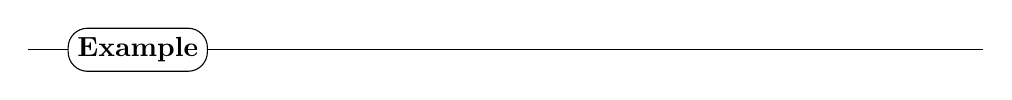
\begin{tikzpicture}
  \draw (0,0) -- (5mm,0)
    node(e)[draw,rectangle,rounded corners=.7em,right] {\bf Example};
  \draw (e) -- (\columnwidth,0);
\end{tikzpicture}%
\medskip%
}

% author comment macros
\newcommand\authornote[3]{{\color{#2} \footnote{\color{#2} {#1}: {#3}}}}
\newcommand\todo[1]{{\color{NavyBlue} \footnote{\color{NavyBlue} TODO: {#1}}}}

\newcommand\asolar[1]{\authornote{AS}{BrickRed}{#1}}  % Armando
\newcommand\cel[1]{\authornote{CL}{OliveGreen}{#1}}   % Charles
\newcommand\rch[1]{\authornote{RC}{RoyalPurple}{#1}}  % Rezaul
\newcommand\pga[1]{\authornote{PG}{RawSienna}{#1}}    % Pramod
\newcommand\coa[1]{\authornote{SI}{NavyBlue}{#1}}     % Shachar

% Armando hack
\newif\ifarmando

\ifluatex
\directlua{
    if not (arg == nil) then
      for i,v in pairs(arg) do
        if (v == "armando") then
          tex.print("\string\\armandotrue")
        end
      end
    end
  }
\fi

\newcommand{\hide}[1]{} 
\newcommand{\C}[1]{\lstinline!#1!}
\newcommand {\spc}{\hspace{3pt}}
\newcommand{\spmd}{\textsc{spmd}}
\newcommand{\cegis}{\textsc{cegis}}
\newcommand{\Sketch}{\textsc{Sketch}}
\newcommand{\lang}{\textsc{SyntRec}}
\newcommand{\constr}{\textsc{guc}}
\hyphenation{spmd cegis Sketch MSL Jacobi}

\newcommand{\constraintenv}{\Sigma}
\newcommand{\cfun}{\gamma}
%%% Inference rule things.
\newcommand{\integ}{\mbox{\texttt{int}}}
%%%%%%%%%%%%%%%%%%%%%%%%%%%%%%%%%%%%%%%%%%%
% Macros for the semantics
%%%%%%%%%%%%%%%%%%%%%%%%%%%%%%%%%%%%%%%%%%%

\newcommand{\valEnv}{\Sigma}
\newcommand{\typeEnv}{\Gamma}
\newcommand{\cdeclEnv}{\Pi}
\newcommand{\cEnv}{\Lambda}

%%%%%%%%%%%%%%%%%%%%%%%%%%%%%%%%%%%%%%%%%%%
%%%%%%%%%%%%%%%%%%%%%%%%%%%%%%%%%%%%%%%%%%

\newcommand{\etal}{\textit{et al.}\@\xspace}
\newcommand{\eg}{\textit{e.g.}\@\xspace}
\newcommand{\ie}{\textit{i.e.}\@\xspace}

% References
%
%\newtheorem{thm}{Theorem}
\newtheorem{lem}{Lemma}
\newtheorem{prop}{Property}

\newcommand{\thmlabel}[1]{\label{thm:#1}}
\newcommand{\thmref}[1]{Theorem~\ref{thm:#1}}
\newcommand{\lemlabel}[1]{\label{lem:#1}}
\newcommand{\lemref}[1]{Lemma~\ref{lem:#1}}

\newcommand{\corlabel}[1]{\label{cor:#1}}
\newcommand{\corref}[1]{Corollary~\ref{cor:#1}}

\newcommand{\proplabel}[1]{\label{prop:#1}}
\newcommand{\propref}[1]{Proposition~\ref{prop:#1}}
\newcommand{\deflabel}[1]{\label{def:#1}}
\newcommand{\defref}[1]{Definition~\ref{def:#1}}
\newcommand{\exlabel}[1]{\label{ex:#1}}
\newcommand{\exref}[1]{Example~\ref{ex:#1}}
\newcommand{\problabel}[1]{\label{prob:#1}}
\newcommand{\probref}[1]{Problem~\ref{prob:#1}}
\newcommand{\obslabel}[1]{\label{obs:#1}}
\newcommand{\obsref}[1]{Observation~\ref{obs:#1}}
\newcommand{\alglabel}[1]{\label{alg:#1}}
%\newcommand{\algref}[1]{Algorithm~\ref{alg:#1}}
%
\newcommand{\applabel}[1]{\label{app:#1}}
\newcommand{\appref}[1]{Appendix~\ref{app:#1}}
\newcommand{\seclabel}[1]{\label{sec:#1}}
\newcommand{\shortsecref}[1]{\S\ref{sec:#1}}
\newcommand{\longsecref}[1]{Section~\ref{sec:#1}}
%
\newcommand{\tablabel}[1]{\label{tab:#1}}
\newcommand{\tabref}[1]{Table~\ref{tab:#1}}
\newcommand{\figlabel}[1]{\label{fig:#1}}
\newcommand{\longfigref}[1]{Figure~\ref{fig:#1}}
\newcommand{\shortfigref}[1]{Fig.~\ref{fig:#1}}
\newcommand{\eqqlabel}[1]{\label{eq:#1}}
\newcommand{\shorteqqref}[1]{\eqref{eq:#1}}
\newcommand{\mediumeqqref}[1]{Eq.~\eqref{eq:#1}}
\newcommand{\longeqqref}[1]{Equation~\eqref{eq:#1}}

% Determine type of references for particular document.
%
\newcommand{\secref}{\longsecref}
\newcommand{\figref}{\longfigref}
\newcommand{\eqqref}{\longeqqref}

% Numbering layout
%
\numberwithin{equation}{section}
\newtheorem{definition}{Definition}
\newtheorem{corollary}{Corollary}
\newtheorem{hypothesis}{Hypothesis}
\newtheorem{algo}{Algorithm}
\newtheorem{Equation}{Equation}
\newtheorem{theorem}{Theorem}[section]


                     %%% Commands for formatting code %%%


% \token -- used for a literal code token
% \nterm -- used for a grammar non-terminal
% Example:  Every \nterm{AssertStmt} begins with the \token{assert} keyword.
\newcommand{\token}[1]{\code{#1}}
\newcommand{\formatnt}[1]{{\sl#1}}  % This _must_ be {\sl#1}, not \textsl{#1}
\newcommand{\nterm}[1]{\index{#1@\formatnt{#1}}\formatnt{#1}}

% syntax -- environment for specifiying syntax
\newenvironment{syntax}
 {\par\begin{tabular}{rcl}}
 {\end{tabular}\vspace{2ex}}

% \lexrule -- used to define a lexical regexp rule within a syntax environment
% Example:  \lexrule{IntegerLiteral}{[0-9]+}
\newcommand{\lexrule}[2]
 {\index{#1@\formatnt{#1}|defpage}\formatnt{#1} &
  $=$ & $\langle${\tt#2}$\rangle$ \\}

% \grammar -- used to define a grammar non-terminal within a syntax environment
% \grammaralt -- used for alternate definitions within a syntax environment
% Example:  \grammar{Expr}{\nterm{Expr} \token{+} \nterm{Expr}}
%           \grammaralt{\token{(} \nterm{Expr} \token{)}}
\newcommand{\grammar}[2]
 {\index{#1@\formatnt{#1}|defpage}\formatnt{#1} & $=$ & {#2} \\}
\newcommand{\grammaralt}[1]{& $|$ & {#1} \\}
\newcommand{\grammarelt}[2]
 {\index{#1@\formatnt{#1}|defpage}\formatnt{#1} & $\in$ & {#2} \\}

\newcommand{\galt}{\mbox{\hspace{0.7em}\ensuremath{|}\hspace{1em}}}

%%% Commands for inserting special characters %%%

% \bs -- used to create a monospace backslash
\newcommand{\bs}{{\tt\char"5C}}

% \us -- used to create a monospace underscore (works better than {\tt\_})
\newcommand{\us}{{\tt\char"5F}}


\usepackage[T1]{fontenc}
%\usepackage[scaled=0.85]{luximono}


\definecolor{dkgreen}{rgb}{0,0.3,0}
\definecolor{gray}{rgb}{0.5,0.5,0.5}
\definecolor{mauve}{rgb}{0.58,0,0.82}
\definecolor{light-gray}{gray}{0.80}

\usepackage{listings}
\lstdefinelanguage{sketch}{
  morekeywords = {
       bool, harness, data, int, bool, adt, new, return, assert , assume, let, case, switch},
  morecomment=[s]{/*}{*/},
}


\lstset{
  language=sketch,
  columns=flexible,
  basicstyle=\fontfamily{lmss}\selectfont\small,
  numbers=none,
  numbersep=3pt,
  numberstyle=\tiny,
  stepnumber=1,
  tabsize=2,
  breaklines=false,
  breakatwhitespace=true,
  commentstyle=\color{cyan},
  mathescape=true,
  escapeinside={\%*}{*)}
}




\renewcommand{\scriptsize}{\fontsize{8.5}{9}\selectfont}
\makeatletter
\lst@AddToHook{TextStyle}{\let\lst@basicstyle\scriptsize\fontfamily{lmss}\selectfont}
\makeatother

\usepackage{url}

\newcommand{\pr}[1]{\left(#1\right)}
\renewcommand{\t}[1]{\text{#1}}
\renewcommand{\b}[1]{\t{\lstinline{#1}}}
\newcommand{\msc}[1]{\ensuremath{\text{{\texttt{#1}}}}}
%\renewcommand{\hss}{\hspace{\stretch{1}}}
\renewcommand{\vss}{\vspace{10pt}}
\newcommand{\sem}[1]{[\![#1]\!]}
\newcommand{\esem}[1]{\mathcal{E}[\![#1]\!]}
\newcommand{\tsem}[1]{\mathcal{T}[\![#1]\!]}
\newcommand{\lam}[2]{\ensuremath{\lambda #1 .\hspace{0.01em} #2}}
\newcommand{\allq}[2]{\ensuremath{\forall #1 .\hspace{0.01em} #2}}
\newcommand{\dbr}[2]{\ensuremath{\{\hspace{-0.2em}| \,#1\,|\,#2\, |\hspace{-0.2em}\}}}
\newcommand{\secsp}{\vspace*{20pt}}

\newcommand{\csubtype}{<:_c}
\newcommand{\fsubtype}{<:_f}
\newcommand{\lub}{\sqcup}
\newcommand{\biglub}{\bigsqcup}
\newcommand{\guard}{\mathcal{G}}

\newcommand{\tenv}{\Gamma}
\newcommand{\denv}{\Delta}
\newcommand{\cenv}{\Sigma}

\newcommand{\stack}[2]{\genfrac{}{}{0pt}{0}{#1}{#2}}

\newcommand{\ors}{\ensuremath{\ |\ \ }}
\newcommand{\deriv}[5]{#1 \vdash \langle #2, #3 \rangle \rightarrow \langle #4, #5 \rangle}
\newcommand{\derivstar}[5]{#1 \vdash \langle #2, #3 \rangle \rightarrow^* \langle #4, #5 \rangle}
\newcommand{\tcrule}[3]{#1 \vdash^c #2 : #3 }
\newcommand{\tdrule}[3]{#1 \vdash #2 : #3}

\newcommand{\nrec}{\stackrel{nr}{\rightarrow}}

% Variables used in symantics and proofs.
\newcommand{\cprim}{c}
\newcommand{\constraint}{\gamma}
\newcommand{\model}{\msc{Model}}
\newcommand{\symbolic}{\sigma}
\newcommand{\store}{\sigma}
\newcommand{\irreducible}{\upsilon}
\newcommand{\levels}{\mathcal{L}}
\newcommand{\lorder}{\sqsubseteq_\levels}
\newcommand{\unsat}{\msc{Unsat}}
\newcommand{\translatesto}{\hookrightarrow}

% For properties...
\newcommand{\spair}[3]{\langle #1 | #2 \rangle_#3}
\newcommand{\cproj}[3]{[#1]_{#2, #3}}

\newcommand{\basetype}{\beta}
\newcommand{\typair}[2]{\langle #1, #2 \rangle}

\def\Cpp{C{}\texttt{++}~}





















\usepackage{rotating}

\usepackage{enumitem}
%\usepackage[breaklinks]{hyperref}

%%\hypersetup{pdfborder={0 0 100}}
%%\usepackage[hyphens]{url}

\newcommand{\lstc}[1]{\text{\lstinline{#1}}}

%\newtheorem{theorem}{Theorem}[section]
\newtheorem{lemma}[theorem]{Lemma}
\newtheorem{proposition}[theorem]{Proposition}
%\newtheorem{corollary}[theorem]{Corollary}
%\newtheorem{definition}[theorem]{Definition}
\newtheorem{example}[theorem]{Example}


\newcommand{\code}[1]{\textsf{#1}}

\newcommand{\conf}[1]{}
\newcommand{\techrep}[1]{#1}

\newcommand{\Mona}{\textsc{Mona}\xspace}

%\newcommand{\Dryad}{\textsc{Dryad}$_\textrm{sep}$\xspace}
%\newenvironment{proof}[1][Proof]{\begin{trivlist}
%\item[\hskip \labelsep {\bfseries #1}]}{\end{trivlist}}
\newcommand{\dryadtree}{\textsc{Dryad}$_\textrm{tree}$\xspace}
\newcommand{\Dryaddec}{\textsc{Dryad}$^\textrm{dec}_\textrm{tree}$\xspace}

%\newcommand{\head}{{\tt head}\xspace}
%\newcommand{\tail}{{\tt tail}\xspace}
%\newcommand{\rroot}{{\tt root}\xspace}
%\newcommand{\nnext}{{\tt next}\xspace}
%\newcommand{\pprev}{{\tt prev}\xspace}
%\newcommand{\loglisthead}{{\tt log\_listhead}\xspace}
%\newcommand{\chname}{{\tt chname}\xspace}
%\newcommand{\filename}{{\tt filename}\xspace}
%\newcommand{\data}{{\tt data}\xspace}

\newcommand{\error}{{\textit{error}}\xspace}
\newcommand{\ffalse}{{{\tt false}}\xspace}
\newcommand{\ttrue}{{{\tt true}}\xspace}
\newcommand{\f}{{\textit{f}}\xspace}
\newcommand{\g}{{\textit{g}}\xspace}


\newcommand{\Dryad}{{\sc Dryad}\xspace}

\newcommand{\head}{{\tt head}\xspace}
\newcommand{\tail}{{\tt tail}\xspace}
\newcommand{\rroot}{{\tt root}\xspace}
\newcommand{\nnext}{{\tt next}\xspace}
\newcommand{\pprev}{{\tt prev}\xspace}
\newcommand{\loglisthead}{{\tt log\_listhead}\xspace}
\newcommand{\chname}{{\tt chname}\xspace}
%\newcommand{\filename}{{\tt filename}\xspace}
\newcommand{\data}{{\tt data}\xspace}
\newcommand{\stmt}{{\tt Stmt}\xspace}
\newcommand{\strfields}{{F}\xspace}

\newcommand{\st}{{\textit st}}
\newcommand{\equal}{{\textit{equal}}}
\newcommand{\dt}{{\textit{dt}}}
\newcommand{\Nadapt}{{\textit Nadapt}}


\newcommand{\adapt}{{\textit{adapt}}}
\newcommand{\Active}{{\textit{active}}}
\newcommand{\nilnode}{{\textit{xnil}}}
\newcommand{\nil}{{\textit{nil}}}
\newcommand{\niltt}{\texttt{nil}\xspace}
\newcommand{\Assume}{{\texttt{assume}}}

\newcommand{\h}{{\textit{h}}}
\newcommand{\rr}{{\textit{r}}}
\newcommand{\p}{{\textit{p}}}
\newcommand{\q}{{\textit{q}}}
\newcommand{\z}{{\textit{z}}}
\newcommand{\x}{{\textit{x}}}
\newcommand{\y}{{\textit{y}}}
\newcommand{\ex}{{\textit{ex}}}
\newcommand{\new}{{\textit{new}}}
\newcommand{\newnode}{{\textit{new}}}
\newcommand{\free}{{\textit{free}}}
\newcommand{\nilvar}{{\textit{nil}}}
\newcommand{\undefined}{{\textit{ndef}}}
\newcommand{\Var}{{\textit{Var}}}

\renewcommand{\implies}{\Rightarrow}

\newcommand{\tuple}[1]{\langle #1 \rangle}
%\newcommand{\ignore}[1]{}
\newcommand{\pc}{\textit{pc}}
\newcommand{\Goal}{\mbox{\textit{Target}}}
\newcommand{\Loc}{\textit{Local}}
\newcommand{\G}{\textit{Global}}
\newcommand{\PC}{\textit{PC}}
\newcommand{\Params}{\mbox{\textit{Par}}}
\newcommand{\atomic}{\mbox{\textit{atom}}}

\newcommand{\calP}{{\cal P}}
\newcommand{\eager}{\mbox{Eager}}
%\newcommand{\qed}{\hfill \mbox{\raggedright \rule{.07in}{.1in}}}

\newcommand{\Strand}{{\sc Strand}\xspace}
\newcommand{\Stranddecsem}{{\sc Strand}\ensuremath{_\textit{dec}^\textit{sem}}\xspace}
\newcommand{\Stranddec}{{\sc Strand}\ensuremath{_\textit{dec}^\textit{syn}}\xspace}
\newcommand{\Stranddecbold}{{\bfseries\scshape Strand}\ensuremath{_\textit{\bfseries dec}^\textit{\bfseries sem}}}
\newcommand{\Stranddecsyn}{{\sc Strand}\ensuremath{_\textit{dec}^\textit{syn}}\xspace}
\newcommand{\Stranddecsynbold}{{\scshape \bfseries Strand}\ensuremath{_\textit{\bfseries dec}}}
\newcommand{\Stranddectree}{{\sc Strand}\ensuremath{_\textit{dec}^{\textit{tree}}}}
\newcommand{\ValidSubmodel}{\textit{ValidSubModel}}
\newcommand{\Subtree}{\textit{Subtree}}
\newcommand{\Graph}{\textit{Graph}}

\newcommand{\SH}{\textit{SH}}
\newcommand{\df}{\textit{df}}
\newcommand{\edf}{f}
\newcommand{\DF}{\textit{DF}}
\newcommand{\pv}{\textit{pv}}
\newcommand{\PV}{\textit{PV}}
\newcommand{\pre}{\textit{pre}}
\newcommand{\post}{\textit{post}}
\newcommand{\dir}{\textit{dir}}
\newcommand{\edir}{d}
\newcommand{\Dir}{\textit{PF}}
\newcommand{\FP}{\textit{F\!P}}
\newcommand{\old}{\textit{old}}
\newcommand{\Def}{\textit{Def}}
\newcommand{\base}{\textit{base}}
\newcommand{\ind}{\textit{ind}}
\newcommand{\aexpr}{\textit{aexpr}}
\newcommand{\bexpr}{\textit{bexpr}}
\newcommand{\TS}{\textit{T\!S}}
\newcommand{\ts}{\textit{ts}}
\newcommand{\Cc}{{C^c}}
\newcommand{\ccnil}{{c_{\textit nil}^c}}
\newcommand{\dirc}{{\textit{dir}^c}}
\newcommand{\dfc}{{\textit{df}^c}}
\newcommand{\pvc}{{\textit{pv}^c}}

\newcommand{\expand}{\textit{expand}}
\newcommand{\funrestrict}[2]{{#1} \mid_{#2}}
\newcommand{\funsubst}[3]{{#1}[{#2} \leftarrow {#3}]}
\newcommand{\formsubst}[3]{{#1}[{#2} / {#3}]}


\newcommand{\key}{\textit{key}}
\newcommand{\keys}{\textit{keys}}
\newcommand{\bst}{\textit{bst}}
\newcommand{\LEFT}{\textit{left}}
\newcommand{\RIGHT}{\textit{right}}

\newcommand{\pf}{\textit{pf}}
\newcommand{\PF}{\textit{PF}}
\newcommand{\vect}[1]{\,\overrightarrow{\!\!#1}}
\newcommand{\ret}{\textit{ret}}
\newcommand{\precall}{\textit{pre\_call}}
\newcommand{\postcall}{\textit{post\_call}}
\newcommand{\precallName}[1]{\textit{pre\_call}\_{#1}}
\newcommand{\postcallName}[1]{\textit{post\_call}\_{#1}}
\newcommand{\vc}{\textit{vc}}
\newcommand{\reachNodes}{\textit{reach\_nodes}}
\newcommand{\treeNodes}{\textit{tree\_nodes}}
%\newcommand{\fresh}[1]{{#1}_\textit{fresh}}
\newcommand{\fresh}[1]{\textit{fresh}\_{#1}}
\newcommand{\oldName}[1]{{#1}_\textit{old}}

\newcommand{\scope}{\text{scope}}
\newcommand{\heapless}{\text{pure}}
\newcommand{\reach}{\text{reachset}}
\newcommand{\tight}{\text{dom-ext}}


\newcommand{\Deref}{\textit{Deref}}
\newcommand{\Mod}{\textit{Mod}}
%\newcommand{\Call}{\textit{Call}}
%\newcommand{\Return}{\textit{Return}}
\newcommand{\footprint}{\textit{fp}}
\newcommand{\rec}{\textit{rec}}


\newcommand{\assume}{\texttt{assume }}
\newcommand{\assert}{\texttt{assert }}
\newcommand{\fpre}{\varphi_\textit{pre}}
\newcommand{\fpost}{\varphi_\textit{post}}
%\newcommand{\nil}{\texttt{nil}}
\newcommand{\emp}{\texttt{emp}}
\newcommand{\true}{\texttt{true}}
\newcommand{\sep}{*}
\newcommand{\lf}{\textit{left}}
\newcommand{\rf}{\textit{right}}
\newcommand{\kf}{\textit{key}}
\newcommand{\rkeys}{\textit{keys}^\dlt_{\vect{\pf}}}
\newcommand{\defrkeys}{\textbf{\textit{keys}}^{\tiny\dlt}_{\tiny\vect{\pf}}}
\newcommand{\figrkeys}{\textit{keys}^{\tiny\dlt}_{\tiny\vect{\pf}}}
\newcommand{\heap}{\textit{mheap}^\dlt_{\vect{\pf}}}
\newcommand{\defheap}{\textbf{\textit{mheap}}^{\tiny\dlt}_{\tiny\vect{\pf}}}
\newcommand{\figheap}{\textit{mheap}^{\tiny\dlt}_{\tiny\vect{\pf}}}
\newcommand{\Logic}{\textsf{DRYAD}}
\newcommand{\reachex}{\textit{reach}_{\{ \lf, \rf \}}}
\newcommand{\GHpre}{G_{pre}}
\newcommand{\GHpost}{G_{post}}
\newcommand{\GH}{G}
\newcommand{\lx}{\textit{lx}}
\newcommand{\rx}{\textit{rx}}

\newcommand{\dlt}{\Delta}

\newcommand{\Stefanescu}{{\c S}tef{\u a}nescu\xspace}

\newcommand{\CopyVars}{{\mathit CopyVars}}
\newcommand{\CopyVarsExcept}{{\mathit CopyVarsExcept}}
\newcommand{\CopyStrFields}{{\mathit CopyStrFields}}
\newcommand{\CopyStrFieldsExcept}{{\mathit CopyStrFieldsExcept}}
\newcommand{\CopyActiveNodes}{{\mathit CopyActiveNodes}}
\newcommand{\CopyActiveNodesExcept}{{\mathit CopyActiveNodesExcept}}
\newcommand{\CopyDataFields}{{\mathit CopyDataFields}}
\newcommand{\CopyDataFieldsExcept}{{\mathit CopyDataFieldsExcept}}
\newcommand{\vcdryadurl}{http://www.cs.illinois.edu/~madhu/vcdryad}

\newcommand{\vcdryad}{\textsc{VCDryad}\xspace}
\newcommand{\vcc}{\textsc{Vcc}\xspace}
\newcommand{\boogie}{\textsc{Boogie}\xspace}
